%*****************************************
\chapter{Working With Data}\label{ch07:data}
%*****************************************

Excel is designed to work with data, and this chapter demonstrates how data is imported and then analyzed with tools like pivot tables. Also included in this chapter is information about safeguarding data and performing two different what-if analysis techniques. 

\section{Importing Data}

\begin{center}
	\begin{objbox}{Learning Objectives}
		\begin{itemize}
			\setlength{\itemsep}{0pt}
			\setlength{\parskip}{0pt}
			\setlength{\parsep}{0pt}
			
			\item Import data from the web and local files.

		\end{itemize}
	\end{objbox}
\end{center}

To use Excel's powerful tools for analysis, data must first be imported into a spreadsheet. Data can be imported from many sources but two common ones are from the web and from a datafile located on the local computer. Data is very often posted on the web for researchers to use in their projects. The United States federal government, for example, has more than $ 200,000 $ datasets freely available in fields like taxes, crime, trade, education, and dozens of other topics\footnote{See \url{https://www.data.gov/}}. Sometimes, that data can be imported directly into Excel but more often it must be downloaded to a local computer and then imported into Excel from that file. This section demonstrates both of those procedures.

\subsection{Import From the Web}

Data in a table on a website can be imported directly into an Excel workbook. Follow these steps to import data from a website.

\begin{enumerate}
	\item Open a new file with a blank workbook.
	\item Save the file as \fmtWorkbookName{WebData.xlsx}.
	\item Click \fmtRibbonGroup{Get External Data} in the \fmtRibbonTab{Data} tab of the ribbon.
	\item Click \fmtPopupButton{From Web} in the popup menu, as shown in Figure \ref{07:fig01}.
\end{enumerate}

\begin{figure}[H]
	\centering
	\includegraphics[width=\maxwidth{.95\linewidth}]{gfx/ch07_fig01}
	\caption{Import From Web Menu}
	\label{07:fig01}
\end{figure}

For this exercise, a page on Wikipedia that has several data tables will be used. The URL is: \url{https://en.wikipedia.org/wiki/Largest_airlines_in_the_world}

\begin{enumerate}[resume]
	\item Enter the URL in the \fmtPopupBox{From Web} popup.
	\item Press \fmtPopupButton{GO}
	\item Excel will access the website and open the \fmtPopupBox{Navigator} window, as shown in Figure \ref{07:fig02}.
\end{enumerate}

\begin{figure}[H]
	\centering
	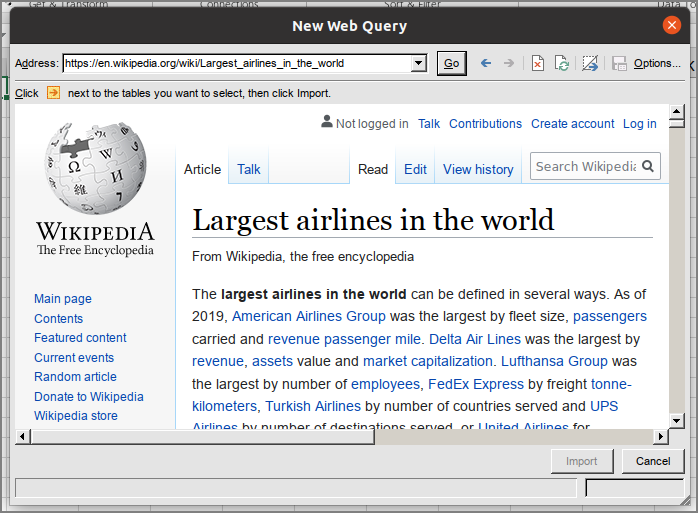
\includegraphics[width=\maxwidth{.95\linewidth}]{gfx/ch07_fig02}
	\caption{From Web URL Window}
	\label{07:fig02}
\end{figure}


\begin{enumerate}[resume]
	\item Scroll down the displayed page until the desired table is visible. Notice a small arrow icon to the left of the table. Click that icon to mark the table for downloading, then click the \fmtPopupButton{Import} button. Figure \ref{07:fig03} shows the data table loaded into Excel.
\end{enumerate}

\begin{figure}[H]
	\centering
	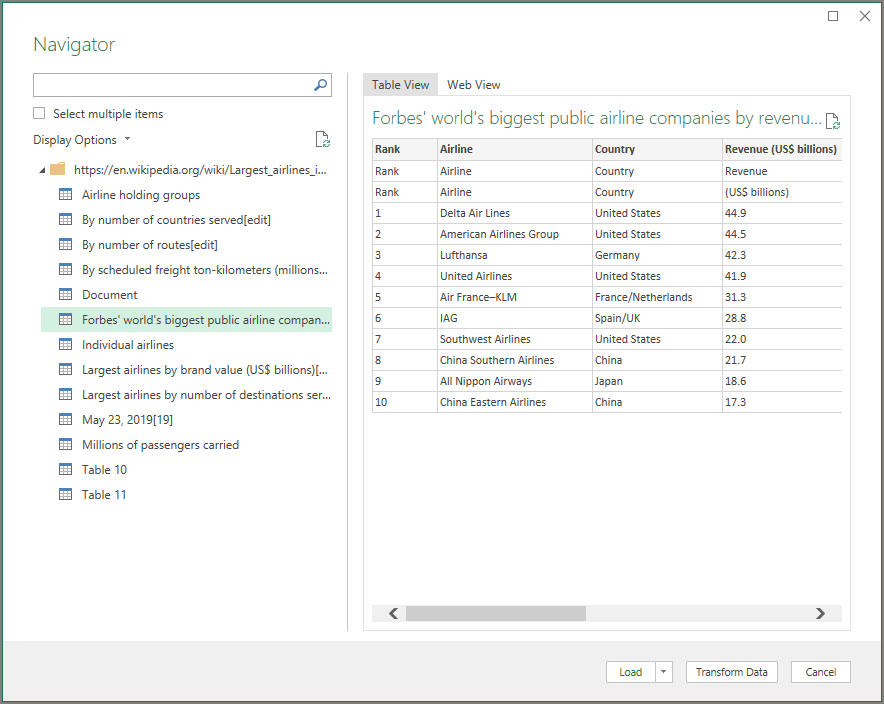
\includegraphics[width=\maxwidth{.95\linewidth}]{gfx/ch07_fig03}
	\caption{Imported Data Table}
	\label{07:fig03}
\end{figure}

Notice that the data is imported into a new worksheet. Excel now displays a \fmtPopupBox{Queries \& Connections} box on the right side of the screen. That box lists the Web queries that were used to import data tables. Since there has only been one query then only one line appears in this box, but if more queries are run they will also be listed here. 

\begin{enumerate}[resume]
	\item Close the \fmtPopupBox{Queries \& Connections} box by clicking the \fmtPopupButton{X} in the top right corner of the box.
\end{enumerate}

A data table is imported into Excel as a table, so tools like filtering, sorting, and slicing the data are readily available. As with any Excel table, this data table can be recolored and formatted as desired. Those skills, though, are taught elsewhere in this class and are not further covered here.

\subsection{Import From Data File}

\textit{Data file: CH7-Data.csv}

It is common for web data to be downloaded via a data file. Those data files are, typically, in a \textit{.CSV} format. This is a simple text file and can be opened with a program no more complicated than Notepad; but they are typically opened with Excel or some other data analysis tool. Figure \ref{07:fig04} shows the first few lines of the sales data file used in this lesson opened in Notepad.

\begin{figure}[H]
	\centering
	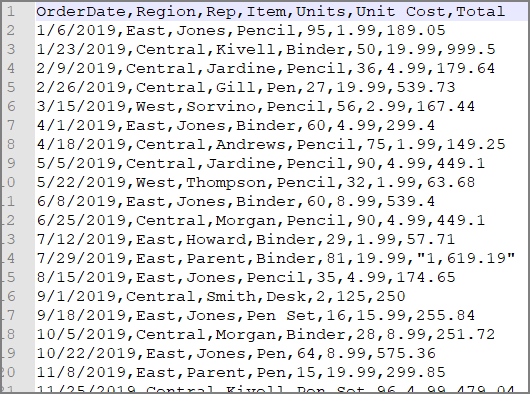
\includegraphics[width=\maxwidth{.95\linewidth}]{gfx/ch07_fig04}
	\caption{CSV File}
	\label{07:fig04}
\end{figure}

Complete the following steps to load a \textit{.CSV} file into Excel.

\begin{enumerate}
	\item Click \fmtRibbonButton{Get External Data} in the \fmtRibbonTab{Data} tab of the ribbon.
	\item Click \fmtPopupButton{From Text}. Figure \ref{07:fig05} illustrates this button.
\end{enumerate}

\begin{figure}[H]
	\centering
	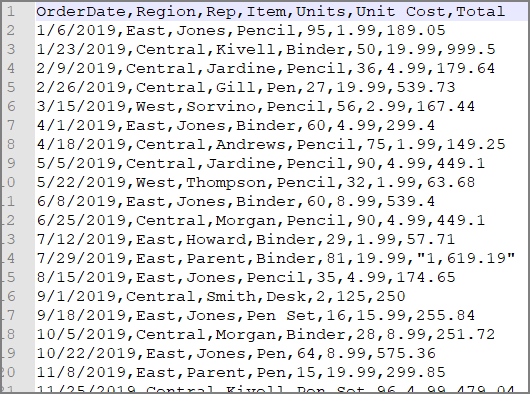
\includegraphics[width=\maxwidth{.95\linewidth}]{gfx/ch07_fig05}
	\caption{Import CSV File}
	\label{07:fig05}
\end{figure}

\begin{enumerate}
	\item Navigate to the data file.
	\item Click the file name and then \fmtPopupButton{Import}. Figure \ref{07:fig06} shows the \fmtPopupBox{Import Text File} dialog box.
\end{enumerate}

\begin{figure}[H]
	\centering
	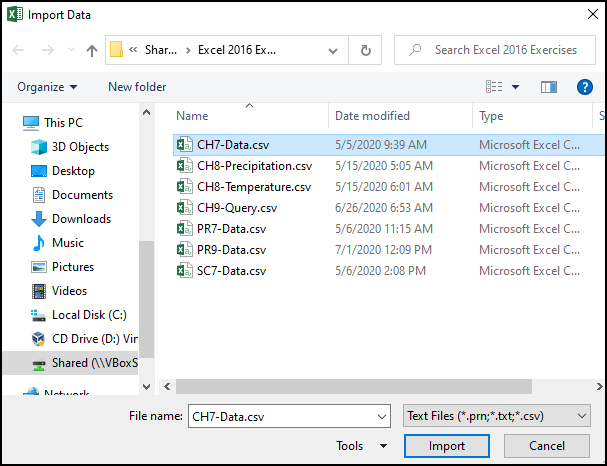
\includegraphics[width=\maxwidth{.95\linewidth}]{gfx/ch07_fig06}
	\caption{Selecting the CSV file}
	\label{07:fig06}
\end{figure}

\begin{enumerate}
	\item Excel will begin to import the .CSV data. Excel starts a wizard that contains its ``best guess'' about the type of data in the file, as illustrated in Figure \ref{07:fig07}.
\end{enumerate}

\begin{figure}[H]
	\centering
	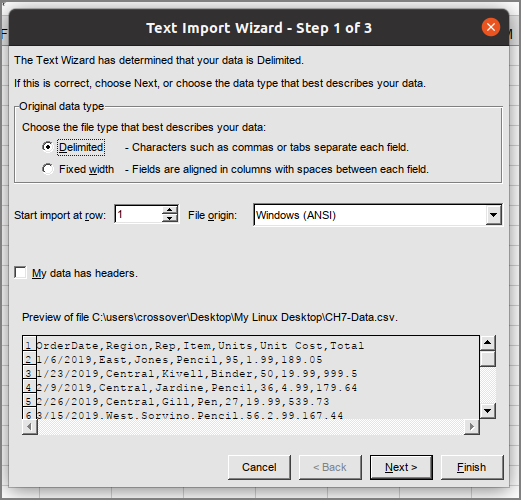
\includegraphics[width=\maxwidth{.95\linewidth}]{gfx/ch07_fig07}
	\caption{Step One of the Text Import Wizard}
	\label{07:fig07}
\end{figure}

\begin{enumerate}
	\item The sample text contained in the box at the bottom of Figure \ref{07:fig07} looks correct, so Excel has correctly determined that the CSV file contains delimited text using Windows format. Click \fmtPopupButton{Next}.
	\item For this data, it is appropriate to begin the import at row 1, but that can be changed if there are several explanatory lines at the top of the file.
	\item Click the \fmtPopupButton{My data has headers} checkbox since the first line of the data contains column headers.
	\item Click \fmtPopupButton{Next}.
	\item Figure \ref{07:fig08} shows that Excel is now guessing that a tab is being used to separate the data columns, but that is not correct. Click the checkbox for \fmtPopupButton{Comma} and notice that the sample data in the box at the bottom of the screen separates into columns.
\end{enumerate}

\begin{figure}[H]
	\centering
	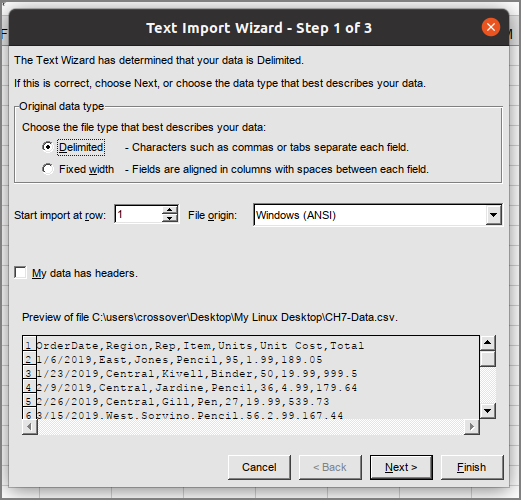
\includegraphics[width=\maxwidth{.95\linewidth}]{gfx/ch07_fig08}
	\caption{Defining Delimiters in the Data Import Wizard}
	\label{07:fig08}
\end{figure}

\begin{enumerate}
	\item Step three of the data import wizard permits users to identify the type of data contained in each column. For this import, click on column one to highlight it and then click on the \fmtPopupButton{Date:} button to define this column as dates. The \textit{MDY} date format option is correct.
	\item Click \fmtPopupButton{Finish} to complete the wizard.
	\item Excel now asks if the data should be loaded into the existing worksheet or create a new worksheet, as illustrated in Figure \ref{07:fig09}.
	\item For this exercise, load the data into cell \fmtCellLocation{A1} in the existing worksheet.
\end{enumerate}

\begin{figure}[H]
	\centering
	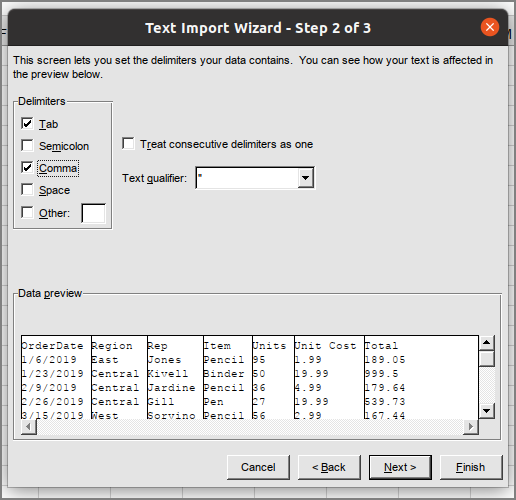
\includegraphics[width=\maxwidth{.95\linewidth}]{gfx/ch07_fig09}
	\caption{Loading the Data}
	\label{07:fig09}
\end{figure}

Figure \ref{07:fig10} shows the first few lines of the worksheet with the imported data.

\begin{figure}[H]
	\centering
	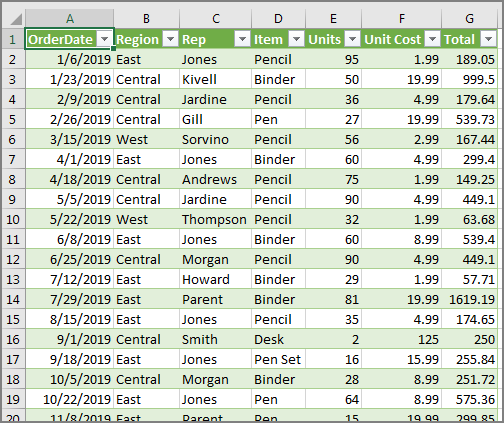
\includegraphics[width=\maxwidth{.95\linewidth}]{gfx/ch07_fig10}
	\caption{The Worksheet With Imported Data}
	\label{07:fig10}
\end{figure}

\begin{enumerate}[resume]
	\item Rename the worksheet to \fmtWorksheetName{Sales Data}.
	\item Save the workbook as \fmtWorkbookName{Sales Summary}.
\end{enumerate}

\begin{center}
	\begin{tkwbox}{Key Take-Aways}
		\textbf{Importing Data}
		\\
		\begin{itemize}
			\setlength{\itemsep}{0pt}
			\setlength{\parskip}{0pt}
			\setlength{\parsep}{0pt}
			
			\item Data can be imported from tables found on websites using \fmtRibbonButton{From Web} on the \fmtRibbonGroup{Get External Data} group on the \fmtRibbonTab{Data} tab on the ribbon.
			\item Data can be imported from CSV files downloaded from websites using \fmtRibbonButton{From Text} on the \fmtRibbonGroup{Get External Data} group on the \fmtRibbonTab{Data} tab on the ribbon.
			
		\end{itemize}
	\end{tkwbox}
\end{center}

\section{Pivot Tables}

\begin{center}
	\begin{objbox}{Learning Objectives}
		\begin{itemize}
			\setlength{\itemsep}{0pt}
			\setlength{\parskip}{0pt}
			\setlength{\parsep}{0pt}

			\item Create a pivot table.
			\item Manipulate a pivot table to change the information displayed.
			
		\end{itemize}
	\end{objbox}
\end{center}

Pivot tables dynamically summarize data and are a favorite tool for analysts since they are highly customizable and very powerful. These tools are called pivot tables because the data displayed can be easily pivoted from rows to columns and back. Pivot tables are sometimes called contingency tables or crosstabs and are frequently seen in reports where tabular data is presented. A common example of a pivot table is found in newspapers and magazines during elections where the editor creates a breakout of voters by party, gender, race, or other factors. For this exercise, sales data from a small supplier will be analyzed.

\begin{enumerate}
	\item Open the \fmtWorkbookName{Sales Summary} workbook if it is not already opened.
	\item Click in cell \fmtCellLocation{A1} in the \fmtWorksheetName{Sales Data} worksheet.
	\item Click \fmtRibbonButton{PivotTable} in the \fmtRibbonGroup{Tables} group on the \fmtRibbonTab{Insert} tab of the ribbon. In Figure \ref{07:fig11}, the \fmtRibbonButton{PivotTable} button can be found at the left end of the ribbon.
\end{enumerate}

\begin{figure}[H]
	\centering
	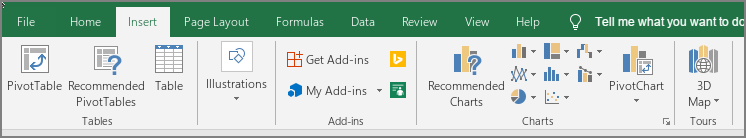
\includegraphics[width=\maxwidth{.95\linewidth}]{gfx/ch07_fig11}
	\caption{PivotTable Button On The Ribbon}
	\label{07:fig11}
\end{figure}

\begin{enumerate}
	\item In the \fmtPopupBox{Create PivotTable} popup, as seen in Figure \ref{07:fig12}, ensure that Excel automatically selected \$A\$1:\$G\$44, which is all the data on the worksheet. Also, ensure \fmtPopupButton{New Worksheet} is selected as the location of the new pivot table. 
	\item Click \fmtPopupButton{OK}.
\end{enumerate}

\begin{figure}[H]
	\centering
	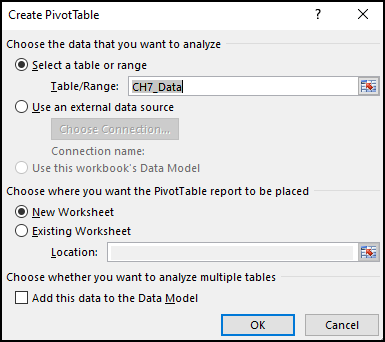
\includegraphics[width=\maxwidth{.95\linewidth}]{gfx/ch07_fig12}
	\caption{Create PivotTable Wizard}
	\label{07:fig12}
\end{figure}


\begin{enumerate}[resume]
	\item A pivot table is created on a new worksheet. Rename that sheet \fmtWorksheetName{Sales Pivot}.
	\item Move the \fmtWorksheetName{Sales Pivot} worksheet to the right of \fmtWorksheetName{Sales Data}.
	\item A blank pivot table has six areas of interest for this lesson, as shown in Figure \ref{07:fig13}.

	\begin{itemize}
		\item \textbf{A}. The \textbf{Pivot Table} will appear in the large area on the left (it is blank in the illustration).
		\item \textbf{B}. The \textbf{Field List} contains the names of all the fields available in the data set. These are the column headers in the data table.
		\item \textbf{C}. \textbf{Filters} is where complex filters can be created to restrict the data displayed on the pivot table.
		\item \textbf{D}. \textbf{Column Labels} define the columns on the pivot table.
		\item \textbf{E}. \textbf{Row Labels} define the rows on the pivot table.
		\item \textbf{F}. \textbf{Values} define the numeric data calculated and displayed in the pivot table.
	\end{itemize}
\end{enumerate}

\begin{figure}[H]
	\centering
	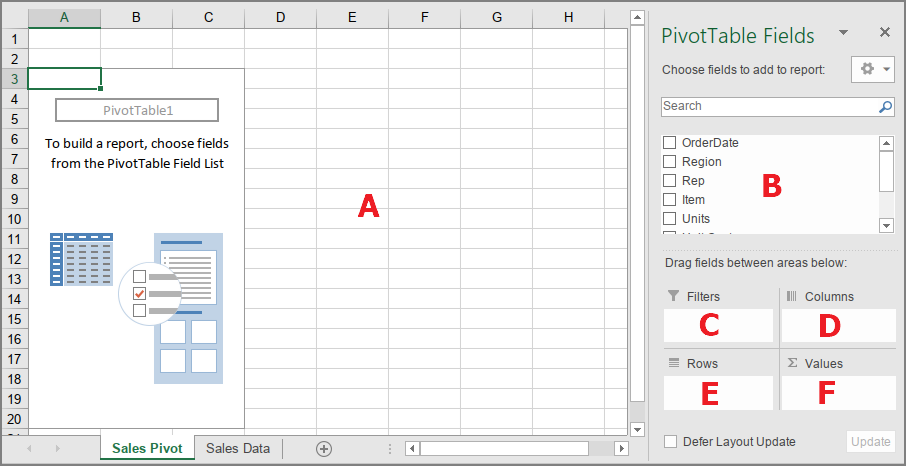
\includegraphics[width=\maxwidth{.95\linewidth}]{gfx/ch07_fig13}
	\caption{Pivot Table Areas}
	\label{07:fig13}
\end{figure}

\begin{enumerate}[resume]
	\item Check the \textit{Region} box in the Field List. By default, Excel places that item in the Row Labels area since it contains text labels. (Note: \textit{Region} can also be dragged to the Row Labels area.)
	\item Check \textit{Item} in the Field List. By default, Excel places Item in the Row Labels area since it contains text labels. (Note: \textit{Item} can also be dragged to the Row Labels area.)
	\item Check \textit{Units} in the Field List. By default, Excel places that Units in the Values area since it contains numbers (notice that Excel automatically creates a sum of Units, but that can be changed to average, max, min, or other statistical values). 
	\item The pivot table now shows how many units of each type of product was sold in each area. There is also a Grand Total at the bottom of the pivot table. With just a few clicks of the mouse, Excel has created a useful decision-making chart for managers. Figure \ref{07:fig14} illustrates the pivot table at this point.
\end{enumerate}

\begin{figure}[H]
	\centering
	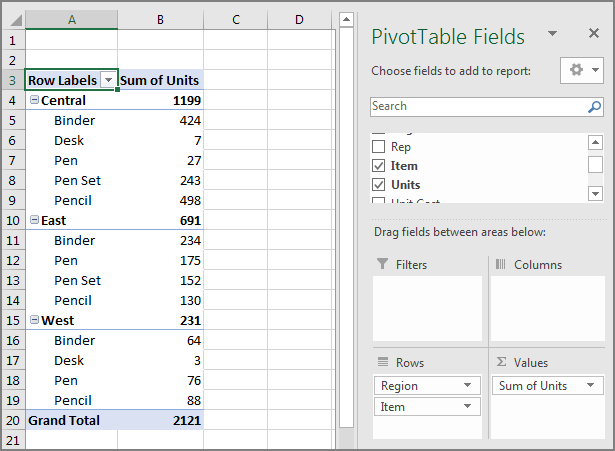
\includegraphics[width=\maxwidth{.95\linewidth}]{gfx/ch07_fig14}
	\caption{Sales Units}
	\label{07:fig14}
\end{figure}
	
\begin{enumerate}[resume]
	\item Click and drag \textit{Item} from the Row Labels area to the Column Labels area. (Note, this can also be done by clicking the down-arrow for \textit{Item} and selecting \fmtPopupButton{Move to Column Labels}.) The same data is still being displayed, but it has been rearranged to make it easier to compare regions. Also notice that Excel automatically created two Grand Totals, one for the rows and one for the columns. Figure \ref{07:fig15} illustrates the pivot table at this point.
\end{enumerate}	

\begin{figure}[H]
	\centering
	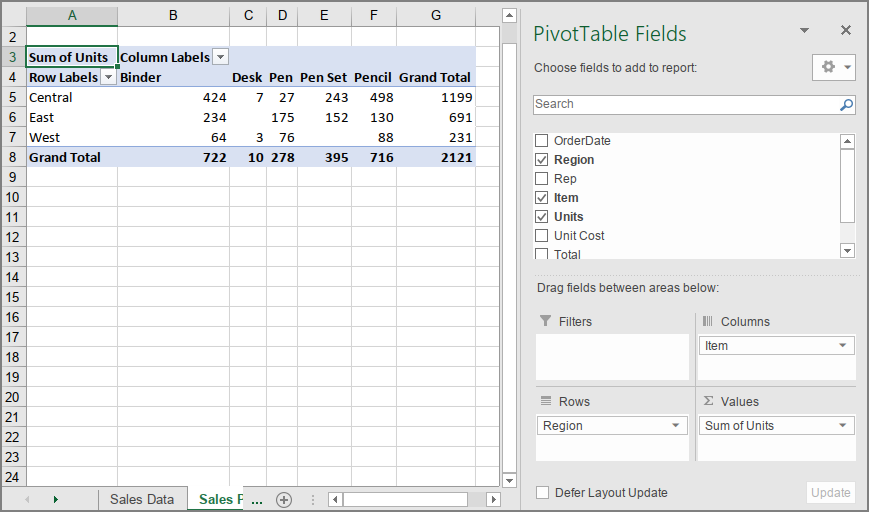
\includegraphics[width=\maxwidth{.95\linewidth}]{gfx/ch07_fig15}
	\caption{Sales Units With Columns}
	\label{07:fig15}
\end{figure}

\begin{enumerate}[resume]
	\item Uncheck \textit{Units} in the Field List. This removes it from the pivot table and leaves only labels with no numbers.
	\item Check \textit{Total} in the Field List. By default, Excel places that item in the Values area since it contains numbers (notice Excel automatically creates a sum of Total). The table now reports the total value of all sales by region and item.
	\item Change the value displayed to average rather than sum.
	
	\begin{enumerate}[resume]
		\item Click the down arrow in \textit{Sum of Total} in the Values area, as illustrated in Figure \ref{07:fig16}
\end{enumerate}

\begin{figure}[H]
	\centering
	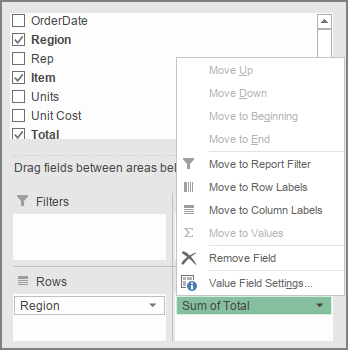
\includegraphics[width=\maxwidth{.95\linewidth}]{gfx/ch07_fig16}
	\caption{Values popup}
	\label{07:fig16}
\end{figure}

\begin{enumerate}[resume]
		\item Select \fmtPopupButton{Value Field Settings}.
		\item Select \fmtPopupButton{Average} in the popup, as illustrated in Figure \ref{07:fig17}
		\item Click \fmtPopupButton{OK}.
\end{enumerate}

\begin{figure}[H]
	\centering
	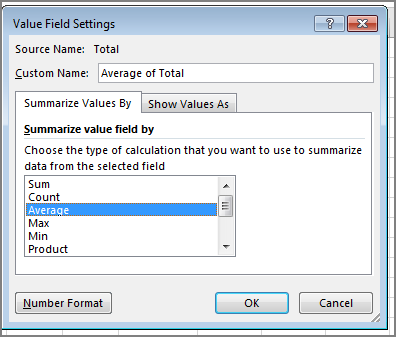
\includegraphics[width=\maxwidth{.95\linewidth}]{gfx/ch07_fig17}
	\caption{Selecting Average Values}
	\label{07:fig17}
\end{figure}

\begin{enumerate}[resume]
		\item The PivotTable is instantly changed to display the average sales by region and item.
	\end{enumerate}

	\item The average is displayed to seven decimal places. Since this is money, it would be best to round the averages to two decimal places.

	\begin{enumerate}[resume]
		\item Click the down arrow in \textit{Average of Total} in the Values area. 
		\item Select \fmtPopupButton{Value Field Settings}.
		\item Click the \fmtPopupButton{Number Format} button at the bottom left corner of the \fmtPopupBox{Value Field Settings} popup, as illustrated in Figure \ref{07:fig18}.
\end{enumerate}

\begin{figure}[H]
	\centering
	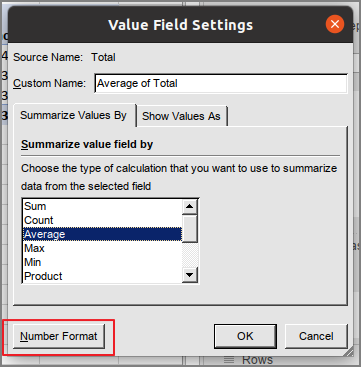
\includegraphics[width=\maxwidth{.95\linewidth}]{gfx/ch07_fig18}
	\caption{The Number Format Button}
	\label{07:fig18}
\end{figure}

\begin{enumerate}[resume]
		\item Choose \fmtPopupButton{Number} and set 2 decimal places (the default setting).
\end{enumerate}

\begin{figure}[H]
	\centering
	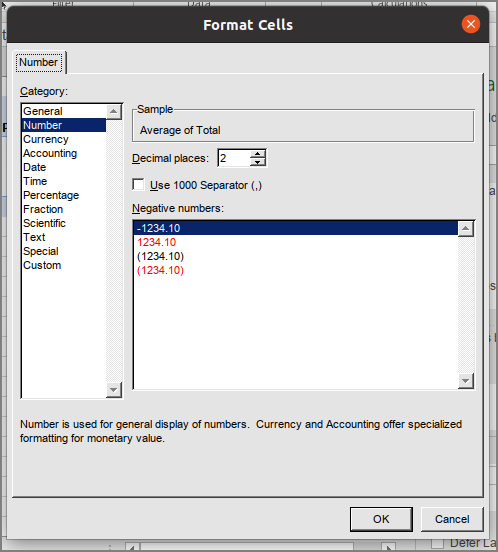
\includegraphics[width=\maxwidth{.95\linewidth}]{gfx/ch07_fig19}
	\caption{Setting Two Decimal Places}
	\label{07:fig19}
\end{figure}

\begin{enumerate}[resume]
		\item Click \fmtPopupButton{OK}.
		\item Click \fmtPopupButton{OK}.
		\item The pivot table is instantly changed to display the averages rounded to two decimal places.
	\end{enumerate}
	
	\item Rename the pivot table by clicking \fmtRibbonButton{PivotTable} in the \fmtRibbonTab{Analyze} tab of the ribbon. Enter \fmtTyping{Sales} for the PivotTable Name, as illustrated in Figure \ref{07:fig20}.
\end{enumerate}

\begin{figure}[H]
	\centering
	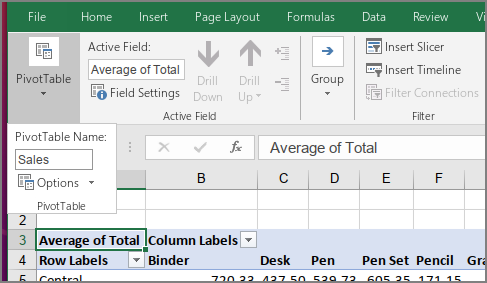
\includegraphics[width=\maxwidth{.95\linewidth}]{gfx/ch07_fig20}
	\caption{Renaming the Pivot Table}
	\label{07:fig20}
\end{figure}

\begin{enumerate}[resume]
	\item Create a new pivot table by clicking in cell \fmtCellLocation{A1} in the \fmtWorksheetName{Sales Data} worksheet.
	\item Click \fmtRibbonButton{PivotTable} in the \fmtRibbonGroup{Tables} group on the \fmtRibbonTab{Insert} tab of the ribbon. 
	\item In the \fmtPopupBox{Create PivotTable} popup, ensure that Excel automatically selected \$A\$1:\$G\$44, which is all the data on the worksheet. Also, ensure \fmtPopupButton{New Worksheet} is selected as the location of the new pivot table. 
	\item Click \fmtPopupButton{OK}.
	\item A pivot table is created on a new worksheet. Rename that worksheet \fmtWorksheetName{Annual Pivot} and move it to the right of \fmtWorksheetName{Sales Pivot}.
	\item Rename the pivot table by clicking \fmtRibbonButton{PivotTable} in the \fmtRibbonTab{Analyze} tab of the ribbon. Enter \fmtTyping{Annual} for the pivot table Name.
	\item Check \textit{OrderDate} in the Field List. By default, Excel places that item in the pivot table Row Labels area since it contains dates. Notice that Excel automatically expands the dates into years, quarters, and months.
	\item Drag \textit{Total} from the Field List to Values. The pivot table now shows the total sales by date. Clicking the plus sign beside the years and quarters in the pivot table drills down to specific quarters and months of interest.
	\item Drag \textit{Region} from the Field List to Columns. This creates columns for each region in the pivot table so now management can find sales by month and region.
	\end{enumerate}	

	\begin{figure}[H]
	\centering
	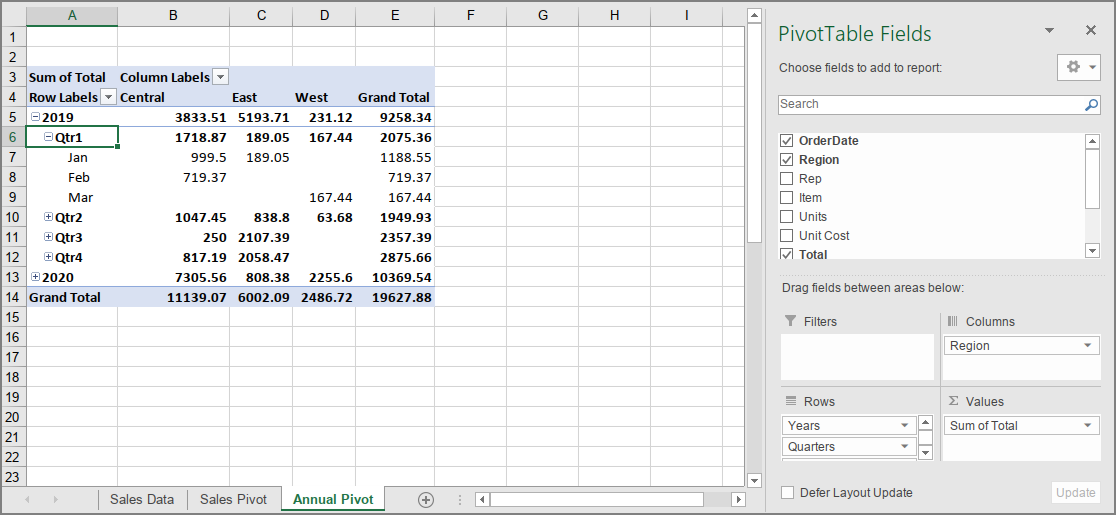
\includegraphics[width=\maxwidth{.95\linewidth}]{gfx/ch07_fig21}
	\caption{Sales Units With Columns}
	\label{07:fig21}
	\end{figure}

	\begin{enumerate}[resume]
	\item To filter the data, click the down arrow to the right of the \textit{Column Labels} or \textit{Row Lables} headers. Check only those regions or dates that should be included in the pivot table. For example, click the down arrow to the right of the \textit{Column Labels} and uncheck everything except \textit{East} and notice how the pivot table is updated to include only the East region. Also notice that the dropdown includes options to sort the data in the pivot table.
\end{enumerate}

\begin{figure}[H]
	\centering
	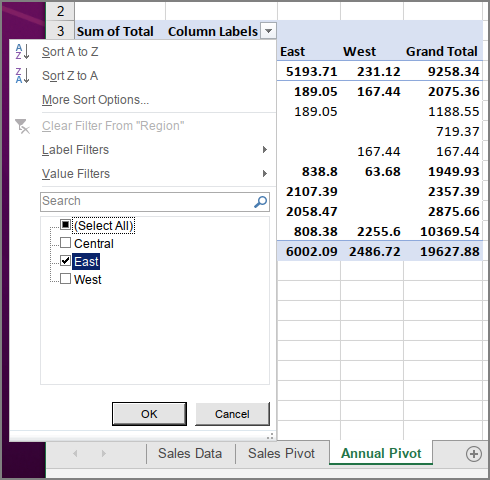
\includegraphics[width=\maxwidth{.95\linewidth}]{gfx/ch07_fig22}
	\caption{Filtering Regions}
	\label{07:fig22}
\end{figure}

\begin{enumerate}[resume]
	\item While managers normally like having dates grouped by month/quarter/year, that can be easily modified. Click cell \fmtCellLocation{A5} in the pivot table so only that one cell is selected. Click the \fmtRibbonButton{Group Field} button in the \fmtRibbonGroup{Group} group in the \fmtRibbonTab{Analyze} tab.
\end{enumerate}

\begin{figure}[H]
	\centering
	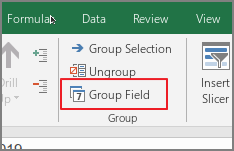
\includegraphics[width=\maxwidth{.95\linewidth}]{gfx/ch07_fig23}
	\caption{The Group Field Button}
	\label{07:fig23}
\end{figure}

\begin{enumerate}[resume]
	\item In the \fmtPopupBox{Grouping} popup box the start/end dates for the data can be specified in order to limit the data shown in the pivot table. For this excercise, leave the dates at their default (two entire years), but click \textit{months} so it is no longer highlighted then click \fmtPopupButton{OK}. Figure \ref{07:fig24} illustrates the \fmtPopupBox{Grouping} popup box after the \fmtPopupButton{Months} item is inactivated. This will remove the \textit{Months} drill down capability and only show years and quarters in the pivot table. By using this option, details can be removed from the pivot table so trends may become more visible.
\end{enumerate}

\begin{figure}[H]
	\centering
	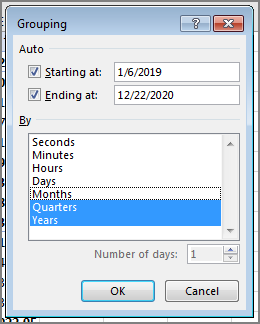
\includegraphics[width=\maxwidth{.95\linewidth}]{gfx/ch07_fig24}
	\caption{Removing Months From The Group}
	\label{07:fig24}
\end{figure}

\begin{enumerate}[resume]
	\item Drag \textit{Rep} from the Field List to the Filters area. Notice that the pivot table now has a selector in cell \fmtCellLocation{B1} so a specific representative (or group of representatives) can be used to filter data on the pivot table. Click the down arrow for the \textit{Rep} filter, select \fmtPopupButton{Andrews}, and click \fmtPopupButton{OK}. Notice that the pivot table is instantly updated to include only Andrews' sales data.
\end{enumerate}

\begin{figure}[H]
\centering
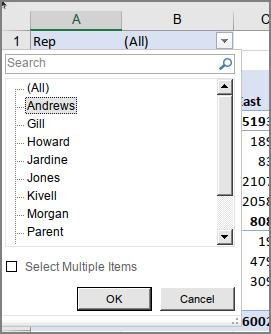
\includegraphics[width=\maxwidth{.95\linewidth}]{gfx/ch07_fig25}
\caption{Filtering For One Representative}
\label{07:fig25}
\end{figure}

\begin{enumerate}[resume]
	\item This pivot table will be used to create a pivot chart in the next section; however, the filter is not needed. Uncheck \textit{Rep} in the Field List to remove that from the filter area.
	\item Save the workbook.
\end{enumerate}

\begin{center}
	\begin{tkwbox}{Key Take-Aways}
		\textbf{Pivot Tables}
		\\
		\begin{itemize}
			\setlength{\itemsep}{0pt}
			\setlength{\parskip}{0pt}
			\setlength{\parsep}{0pt}
			
			\item Pivot tables are a very powerful analysis tool that are easy to create and use.
			
		\end{itemize}
	\end{tkwbox}
\end{center}

\section{Recommended Pivot Tables}

\begin{center}
	\begin{objbox}{Learning Objectives}
		\begin{itemize}
			\setlength{\itemsep}{0pt}
			\setlength{\parskip}{0pt}
			\setlength{\parsep}{0pt}
			
			\item Evaluate and select a recommended pivot table.
			
		\end{itemize}
	\end{objbox}
\end{center}

\begin{enumerate}
	\item Open the \fmtWorkbookName{Sales Summary} workbook.
	\item Click cell \fmtCellLocation{A1} in the \fmtWorksheetName{Sales Data} worksheet.
	\item Click \fmtRibbonButton{Recommended PivotTables} in the \fmtRibbonGroup{Tables} group of the \fmtRibbonTab{Insert} tab.
	\item Excel will analyze the data and create several recommended pivot tables. These can be clicked and previewed in the \fmtPopupBox{Recommended PivotTables} popup. Figure \ref{07:fig26} illustrates the \fmtPopupBox{Recommended PivotTables} popup.
\end{enumerate}

\begin{figure}[H]
	\centering
	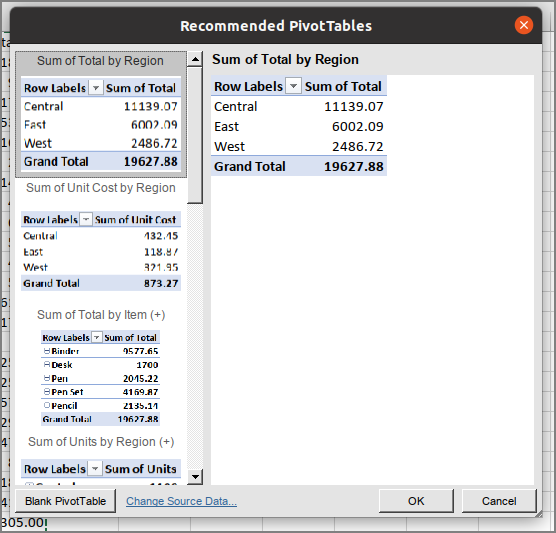
\includegraphics[width=\maxwidth{.95\linewidth}]{gfx/ch07_fig26}
	\caption{Recommended PivotTables}
	\label{07:fig26}
\end{figure}

\begin{enumerate}[resume]
	\item Click on the first recommended pivot table, \fmtPopupButton{Sum of Total by Region}, and click \fmtPopupButton{OK}.
	\item Excel creates the pivot table in a new worksheet. Name that worksheet \fmtWorksheetName{Sales By Region}.
	Move \fmtWorksheetName{Sales By Region} to the right of \fmtWorksheetName{Annual Pivot}.
	\item Rename the pivot table by clicking \fmtRibbonButton{PivotTable} in the \fmtRibbonTab{Analyze} tab of the ribbon. Enter \fmtTyping{By Region} for the PivotTable Name.	
	\item The new pivot table includes all of the same features as those created manually so formatting and variable manipulation is available to modify this table.
\end{enumerate}

\begin{center}
	\begin{tkwbox}{Key Take-Aways}
		\textbf{Recommended Pivot Tables}
		\\
		\begin{itemize}
			\setlength{\itemsep}{0pt}
			\setlength{\parskip}{0pt}
			\setlength{\parsep}{0pt}
			
			\item Excel automatically analyzes data in a worksheet and recommends appropriate pivot tables for the data.
			\item If a recommended pivot table is selected, it can be easily manipulated to meet the goals of the research project.
			
		\end{itemize}
	\end{tkwbox}
\end{center}

\section{Pivot Charts}

\begin{center}
	\begin{objbox}{Learning Objectives}
		\begin{itemize}
			\setlength{\itemsep}{0pt}
			\setlength{\parskip}{0pt}
			\setlength{\parsep}{0pt}
			
			\item Create and format a pivot chart.
			
		\end{itemize}
	\end{objbox}
\end{center}

One of the strengths of creating a pivot table is that the table can be used to create a chart and as the table is modified the chart is also automatically modified. Follow these directions to explore the power of pivot charts.

\begin{enumerate}
	\item Open the \fmtWorksheetName{Sales Data} worksheet in the \fmtWorkbookName{Sales Summary} workbook.
	\item Activate cell \fmtCellLocation{A1} by clicking in it.  
	\item Click \fmtRibbonButton{Pivot Chart} in the \fmtRibbonGroup{Charts} group of the \fmtRibbonTab{Insert} tab.
\end{enumerate}

\begin{figure}[H]
	\centering
	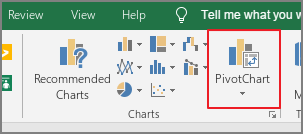
\includegraphics[width=\maxwidth{.95\linewidth}]{gfx/ch07_fig27}
	\caption{The Pivot Chart Button}
	\label{07:fig27}
\end{figure}

\begin{enumerate}[resume]	
	\item In the \fmtPopupBox{Create PivotChart} popup, ensure that Excel automatically selected \$A\$1:\$G\$44, which is all the data on the worksheet. Also, ensure \fmtPopupButton{New Worksheet} is selected as the location of the new pivot chart.
	\item Click \fmtPopupButton{OK}.
	\item Excel will open a new pivot chart worksheet. This worksheet is similar to a pivot table worksheet and creating a chart is like creating a table.
	\item Rename the pivot chart worksheet to \fmtWorksheetName{Sales By Item}. 
	\item Move \fmtWorksheetName{Sales By Item} to the right of \fmtWorksheetName{Sales By Region}.
	\item Select \fmtPopupButton{Rep} and \fmtPopupButton{Total}. Excel creates a bar chart that shows the total sales for each Representative, as illustrated in Figure \ref{07:fig28}.
\end{enumerate}	

\begin{figure}[H]
	\centering
	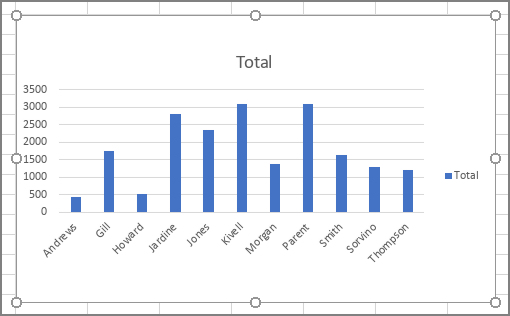
\includegraphics[width=\maxwidth{.95\linewidth}]{gfx/ch07_fig28}
	\caption{Sales By Representative}
	\label{07:fig28}
\end{figure}

\begin{enumerate}
	\item Uncheck \fmtPopupButton{Rep} and check \fmtPopupButton{Item}.
	\item The bar chart automatically updates to display the total sales for each item in the inventory. This chart, though, would be better if it were a pie chart.
	
	\begin{enumerate}
		\item Click the down arrow for the \fmtPopupButton{Sum of Total} item in the \textit{Values} area of the pivot table.
		\item Select \fmtPopupButton{Value Field Settings} in the popup options menu.
		\item Click the \fmtPopupButton{Show Values As} tab in the \fmtPopupBox{Value Field Settings} popup box.
		\item Choose \fmtPopupButton{\% of Grand Total} in the drop-down menu near the middle of the \fmtPopupBox{Value Field Settings} box.
\end{enumerate}

\begin{figure}[H]
	\centering
	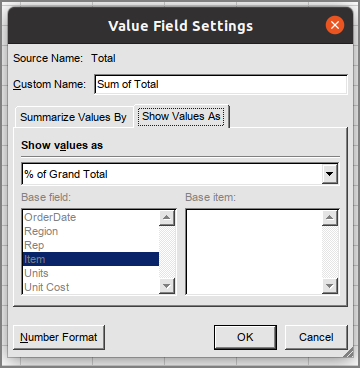
\includegraphics[width=\maxwidth{.95\linewidth}]{gfx/ch07_fig29}
	\caption{Values As a Percentage Of The Total}
	\label{07:fig29}
\end{figure}

\begin{enumerate}[resume]		
		\item Click \fmtPopupButton{OK}.
		\item The values in the pivot table change to percentages rather than numbers.
	\end{enumerate}
	
	\item Click \fmtRibbonButton{Change Chart Type} in the \fmtRibbonGroup{Type} group of the \fmtRibbonTab{Design} tab on the ribbon.
	\item Select \fmtPopupButton{Pie Chart} and click \fmtPopupButton{OK}.
\end{enumerate}

\begin{figure}[H]
	\centering
	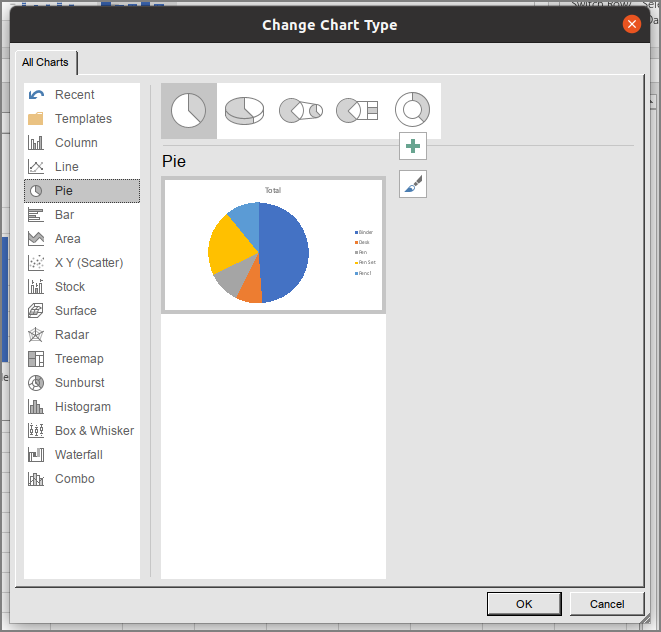
\includegraphics[width=\maxwidth{.95\linewidth}]{gfx/ch07_fig30}
	\caption{Selecting a Pie Chart}
	\label{07:fig30}
\end{figure}

\begin{enumerate}[resume]	
	\item Click the $ + $ sign at the top right of the pie chart and then click \fmtPopupButton{Data Labels} to display the percent of each slice.
\end{enumerate}

\begin{figure}[H]
	\centering
	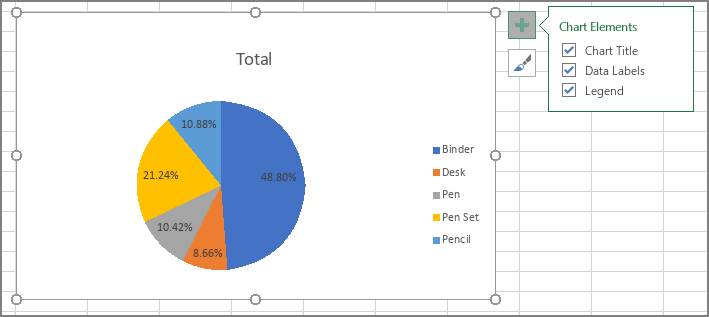
\includegraphics[width=\maxwidth{.95\linewidth}]{gfx/ch07_fig31}
	\caption{Adding Data Labels}
	\label{07:fig31}
\end{figure}

\begin{enumerate}[resume]	
	\item Click off of the chart so it is no longer selected and then right-click on the chart title. Select \fmtPopupButton{Edit Text} from the popup menu.
\end{enumerate}

\begin{figure}[H]
	\centering
	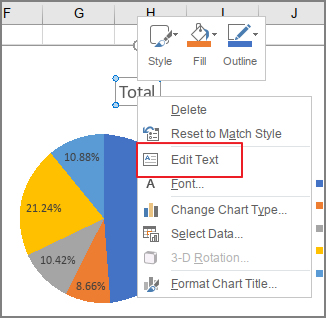
\includegraphics[width=\maxwidth{.95\linewidth}]{gfx/ch07_fig32}
	\caption{Editing The Title}
	\label{07:fig32}
\end{figure}

\begin{enumerate}[resume]	
	\item Enter \fmtTyping{Sales by Item} as the chart title and then click off of the chart so it is no longer selected.
	\item The chart colors and other chart elements can be changed using options found on the \fmtRibbonTab{Design} tab.
	\item Save the workbook.
\end{enumerate}

\begin{center}
	\begin{tkwbox}{Key Take-Aways}
		\textbf{Pivot Charts}
		\\
		\begin{itemize}
			\setlength{\itemsep}{0pt}
			\setlength{\parskip}{0pt}
			\setlength{\parsep}{0pt}
			
			\item Creating a pivot chart uses the same process as a pivot table.
			\item Once a pivot chart has been created, it can be modified using all of the chart tools.
			
		\end{itemize}
	\end{tkwbox}
\end{center}

\section{Safeguarding}

\begin{center}
	\begin{objbox}{Learning Objectives}
		\begin{itemize}
			\setlength{\itemsep}{0pt}
			\setlength{\parskip}{0pt}
			\setlength{\parsep}{0pt}
			
			\item Validate data input to decrease typing errors.
			\item Lock worksheet cells, or entire worksheets, so users do not accidentally change or delete formulas.
			
		\end{itemize}
	\end{objbox}
\end{center}

It is occasionally desirable to safeguard certain cells in a worksheet, or the entire worksheet, to keep a user from accidentally changing something important. For example, if several cells include complex formulas then those should be secured so users will not accidentally delete them. There are two methods generally used to safeguard worksheets: data validation and worksheet protection. 

\subsection{Data Validation}

Excel's data validation rules can be used in a variety of ways.

\begin{itemize}
	\item Restrict the data entered into a cell.
	\item Circle all cells that do not conform to specified validation rules.
	\item Limit the user to a list of possibilities.
\end{itemize}

One of the easiest ways to restrict data is to provide a drop-down list of choices for the user. 

\begin{enumerate}
	\item Open \fmtWorkbookName{CH7-Advanced.xlsx}.
	\item Select the \fmtWorksheetName{Validation} worksheet.
	\item Notice that this sheet includes a list of Zip codes in cells \fmtCellLocation{K2:K10}. The goal is to permit the user to only select from this list of Zip codes to help reduce data entry errors.
	\item The first step is to name the list of zip codes.
	
	\begin{enumerate}
		\item Select K2:K10.
		\item Click \fmtRibbonButton{Define Name} in the \fmtRibbonGroup{Defined Names} group on the \fmtRibbonTab{Formulas} tab.
		\end{enumerate}
		
		\begin{figure}[H]
			\centering
			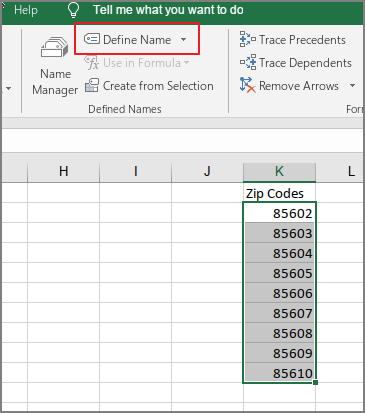
\includegraphics[width=\maxwidth{.95\linewidth}]{gfx/ch07_fig33}
			\caption{Selecting a Range of Cells to Name}
			\label{07:fig33}
		\end{figure}
		
		\begin{enumerate}[resume]		
		\item Name the selected cells \fmtTyping{Zip}.
		\item Click \fmtPopupButton{OK}.
		\begin{figure}[H]
			\centering
			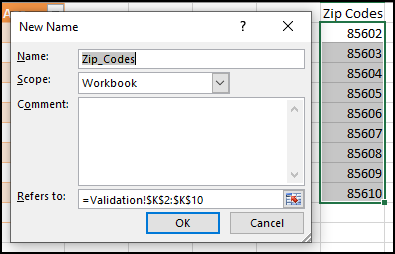
\includegraphics[width=\maxwidth{.95\linewidth}]{gfx/ch07_fig34}
			\caption{Naming a Range of Cells}
			\label{07:fig34}
		\end{figure}
	\end{enumerate}
	
	\item Select \fmtCellLocation{D2}, which is the first cell that needs data validation. 
	\item Click \fmtRibbonButton{Data Validation} on the \fmtRibbonGroup{Data tools} group of the \fmtRibbonTab{Data} tab on the ribbon. (\textit{Note}, click the button, not the down arrow on the right side of the button.)
\end{enumerate}

\begin{figure}[H]
	\centering
	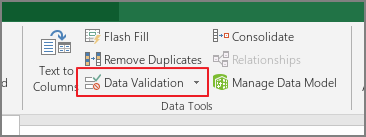
\includegraphics[width=\maxwidth{.95\linewidth}]{gfx/ch07_fig35}
	\caption{The Data Validation Button}
	\label{07:fig35}
\end{figure}

\begin{enumerate}[resume]	
	\item Select \fmtPopupButton{List} in the \fmtPopupBox{Allow} field.
\end{enumerate}

\begin{figure}[H]
	\centering
	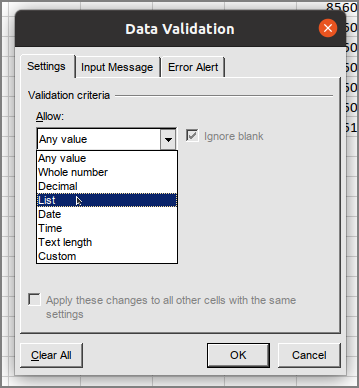
\includegraphics[width=\maxwidth{.95\linewidth}]{gfx/ch07_fig36}
	\caption{Selecting A Validation List}
	\label{07:fig36}
\end{figure}

\begin{enumerate}[resume]	
	\item Check \fmtPopupButton{Ignore blank}. If this is left unchecked then it would force the user to enter a zip code, but when this is checked the user can leave the zip code field blank.
	\item Check \fmtPopupButton{In-cell dropdown}. This creates a drop-down list so the user can select a zip code from a list rather than enter it manually.
	\item Enter \fmtTyping{=Zip} for the \fmtPopupBox{Source}. This tells Excel that the acceptable list of zip codes for cell \fmtCellLocation{D2} is found in the \textit{Zip} list.
	\item Click \fmtPopupButton{OK}.
\end{enumerate}

\begin{figure}[H]
	\centering
	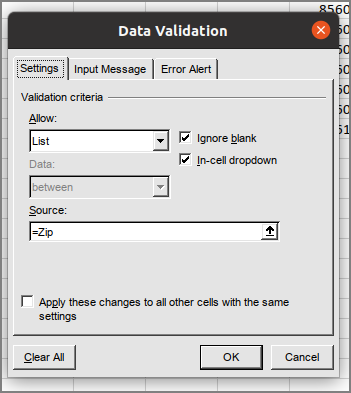
\includegraphics[width=\maxwidth{.95\linewidth}]{gfx/ch07_fig37}
	\caption{Setting the Data Validation List}
	\label{07:fig37}
\end{figure}

After following the above steps, a drop-down selection box will appear whenever the user click into cell \fmtCellLocation{D2}, as illustrated in Figure \ref{07:fig38}. That cell can then be copied to \fmtCellLocation{D3:D6} so all of those cells will get the same drop-down selection.

\begin{figure}[H]
	\centering
	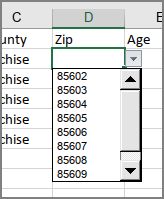
\includegraphics[width=\maxwidth{.95\linewidth}]{gfx/ch07_fig38}
	\caption{Valid Selections}
	\label{07:fig38}
\end{figure}

\begin{center}
	\begin{infobox}{Note}
		\textbf{Validation List Location}
		\\
		\\
		For this exercise the list of valid zip codes was contained on the same worksheet as the cells to be validated. However, the validation list is normally found on a different worksheet so it can be protected and, optionally, hidden from the user.
	\end{infobox}
\end{center}

A second validation method is used when the user can enter data that cannot be selected from a list. For example, if users are required to enter their age then a drop-down list containing every possible age is not reasonable. In this case, Excel can be set up to ensure that the data entered is within certain specific bounds. For example, an ``age'' entry should be between $ 1 $ and $ 99 $ (or maybe some other range). Data validation can use a full set of Boolean comparisons (between, equal to, greater than, etc.). As part of the process, various messages can be displayed when the cell is selected to help guide the user. Finally, the action taken when invalid data is entered (\textit{Stop}, \textit{Warning}, or \textit{Information}) can be specified.

\begin{enumerate}
	\item Open \fmtWorkbookName{CH7-Advanced.xlsx}.
	\item Select the \fmtWorksheetName{Validation} worksheet.
	\item Notice that this sheet includes an entry for Age. The expectation is that users will enter their age but it is important to restrict this data to numbers between $ 1 $ and $ 99 $ so they do not accidentally enter a large number or even text.
	\item Select \fmtCellLocation{E2}, which is the first cell that needs data validation. 
	\item Click \fmtRibbonButton{Data Validation} on the \fmtRibbonGroup{Data tools} group of the \fmtRibbonTab{Data} tab on the ribbon. (\textit{Note}, click the button, not the down arrow on the right side of the button.)
	\item Select \fmtPopupButton{Whole number} in the \fmtPopupBox{Allow} field.
	\item Select \fmtPopupButton{Between} in the \fmtPopupBox{Data} field.
	\item Enter \fmtTyping{1} in the \fmtPopupBox{Minimum} field.
	\item Enter \fmtTyping{99} in the \fmtPopupBox{Maximum} field.
\end{enumerate}

\begin{figure}[H]
	\centering
	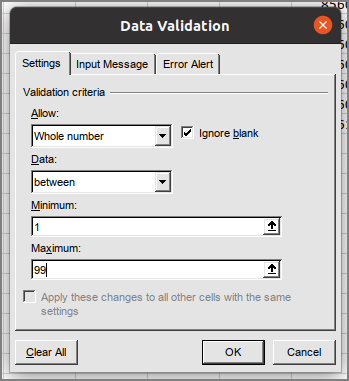
\includegraphics[width=\maxwidth{.95\linewidth}]{gfx/ch07_fig39}
	\caption{Settings for Validating Numeric Data}
	\label{07:fig39}
\end{figure}

\begin{enumerate}[resume]	
	\item Click the \fmtPopupBox{Input Message} tab and enter \fmtTyping{Age} for the \textit{Title} and \fmtTyping{Input an age between $ 1 $ and $ 99 $} for the \textit{Input Message}.
	\item Click the \fmtPopupBox{Error Alert} tab and select the \fmtPopupButton{Stop} style then enter \fmtTyping{Age} for the \textit{Title} and \fmtTyping{Input an age between $ 1 $ and $ 99 $} for the \textit{Input Message}.
	\item Click \fmtPopupButton{OK}.
	\item Copy \fmtCellLocation{E2} to \fmtCellLocation{E3:E6}.
	\item Click in \fmtCellLocation{E2} to activate that cell. Notice that the help message pops up. Enter some number in \fmtCellLocation{E2}. If that number is between $ 1 $ and $ 99 $ then the entry works without error, but if anything else is entered an error message pops up and forces a correct number to be entered.
\end{enumerate}

\begin{figure}[H]
	\centering
	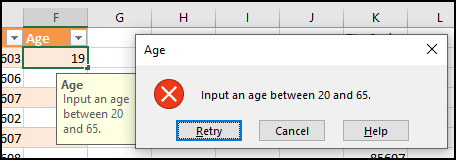
\includegraphics[width=\maxwidth{.95\linewidth}]{gfx/ch07_fig40}
	\caption{Stopping on Data Entry Error}
	\label{07:fig40}
\end{figure}

\begin{enumerate}[resume]	
	\item Click \fmtCellLocation{E2} to activate that cell.
	\item Click \fmtRibbonButton{Data Validation} on the \fmtRibbonGroup{Data tools} group of the \fmtRibbonTab{Data} tab on the ribbon. (\textit{Note}, click the button, not the down arrow on the right side of the button.)
	\item Click the \fmtPopupBox{Error Alert} tab on the \fmtPopupBox{Data Validation} dialog box. 
	\item This cell was initially set to \textit{Stop} on an error. Perhaps, though, it would be acceptable for the user to finish the data entry even if it contained an error. Change the Style drop-down to \fmtPopupButton{Warning}.
	\item Click \fmtPopupButton{OK}.
	\item Copy \fmtCellLocation{E2} to \fmtCellLocation{E3:E6}.
	\item Click in \fmtCellLocation{E2} to activate that cell. Notice that the help message pops up. Enter some number in \fmtCellLocation{E2}. If that number is between $ 1 $ and $ 99 $ then the entry works without error, but if anything else is entered a warning message pops up and permits the user to continue with the bad number or retry.
\end{enumerate}

\begin{figure}[H]
	\centering
	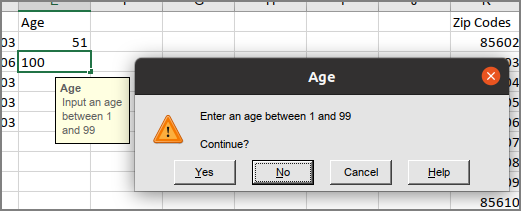
\includegraphics[width=\maxwidth{.95\linewidth}]{gfx/ch07_fig41}
	\caption{Warning on Data Entry Error}
	\label{07:fig41}
\end{figure}

\begin{enumerate}[resume]	
	\item Enter these numbers into cells \fmtCellLocation{E3:E6}: $ 51 $, $ 100 $, $ 40 $, $ 99 $, $ 0 $. A warning should pop up for \fmtCellLocation{E4} and \fmtCellLocation{E6} since those entries are out of the acceptable range, but click \fmtPopupButton{Yes} on the warning popup box so the data is entered.
	\item Click the down arrow on the right side of the \fmtRibbonButton{Data Validation} button in the \fmtRibbonGroup{Data tools} group of the \fmtRibbonTab{Data} tab on the ribbon.
	\item Select \fmtPopupButton{Circle lnvalid Data}.
\end{enumerate}

\begin{figure}[H]
	\centering
	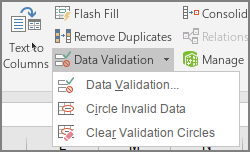
\includegraphics[width=\maxwidth{.95\linewidth}]{gfx/ch07_fig42}
	\caption{Data Validation Options}
	\label{07:fig42}
\end{figure}

\begin{enumerate}[resume]	
	\item Notice that the cells containing bad data are now circled so they can be corrected.
\end{enumerate}

\begin{figure}[H]
	\centering
	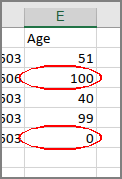
\includegraphics[width=\maxwidth{.95\linewidth}]{gfx/ch07_fig43}
	\caption{Circled Data Errors}
	\label{07:fig43}
\end{figure}

\begin{enumerate}[resume]	
	\item Click the down arrow on the right side of the \fmtRibbonButton{Data Validation} button on the \fmtRibbonGroup{Data tools} group of the \fmtRibbonTab{Data} tab on the ribbon. 
	\item Select \fmtPopupButton{Clear Validation Circles} to clear the validation circles.
\end{enumerate}

\begin{center}
	\begin{infobox}{Note}
		\textbf{Data Validation}
		\\
		\\
		Data validation will not automatically update the error circles as new data is entered. Therefore, after data is entered into a worksheet the \fmtPopupButton{Circle Invalid Data} button must be clicked to check that data.
	\end{infobox}
\end{center}

\subsection{Worksheet Protection}

After entering the data validation rules, it is desired to lock the \fmtWorksheetName{Validation} worksheet so users cannot accidentally delete the formulas. Before adding protection to a worksheet, cells that need to remain open for editing must be unlocked. That way, after the entire sheet is locked those selected cells can still be edited. Follow these steps to unlock cells that should remain editable. 

\begin{enumerate}
	\item Click on the \fmtWorksheetName{Validation} worksheet tab to activate it.
	\item Select \fmtCellLocation{D2:E6}. 
	\item Right-click on the selected cells.
	\item Select \fmtPopupButton{Format Cells} from the popup menu.
	\item Click the \fmtPopupBox{Protection} tab of the dialog box.
	\item Uncheck \fmtPopupButton{Locked}.
	\item Click \fmtPopupButton{OK}.
\end{enumerate}

\begin{figure}[H]
	\centering
	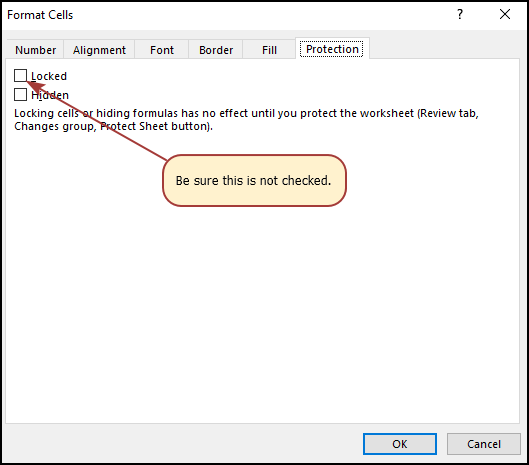
\includegraphics[width=\maxwidth{.95\linewidth}]{gfx/ch07_fig44}
	\caption{Unlocking Editable Cells}
	\label{07:fig44}
\end{figure}

Next, do this to lock the sheet.

\begin{enumerate}
	\item Click \fmtRibbonButton{Protect Sheet} in the \fmtRibbonGroup{Protect} group on the \fmtRibbonTab{Review} tab.
	\item Check \fmtPopupButton{Protect worksheet and contants of locked cells}.
	\item Uncheck all options except \fmtRibbonButton{Select Unlocked Cells}.
	\item Click \fmtPopupButton{OK}.
	\item Notice that now the mouse cannot click in any cell except \fmtCellLocation{D2:E6}
\end{enumerate}

\begin{center}
	\begin{infobox}{Important!}
		\textbf{Password}
		\\
		\\
		Worksheets can be password protected, but there is no way to recover the worksheet if the password is forgotten. Therefore, it is essential to use a password that is easy to remember but difficult to guess.
	\end{infobox}
\end{center}

\begin{center}
	\begin{infobox}{Important!}
		\textbf{Security}
		\\
		\\
		While it is easy to lock worksheets to keep users from accidentally changing a formula, this should not be considered any sort of security. Users can easily unlock the worksheet and make whatever changes they want. This is just a way to stop users from accidentally making changes.
	\end{infobox}
\end{center}

\begin{center}
	\begin{tkwbox}{Key Take-Aways}
		\textbf{Safeguarding}
		\\
		\begin{itemize}
			\setlength{\itemsep}{0pt}
			\setlength{\parskip}{0pt}
			\setlength{\parsep}{0pt}
			
			\item Data entry can be validated to decrease the chance of bad data being entered due to simple typing errors.
			\item Worksheets can be protected so users cannot accidentally change formulas or data.
			
		\end{itemize}
	\end{tkwbox}
\end{center}

\section{What-if Analysis}

\begin{center}
	\begin{objbox}{Learning Objectives}
		\begin{itemize}
			\setlength{\itemsep}{0pt}
			\setlength{\parskip}{0pt}
			\setlength{\parsep}{0pt}
			
			\item Use a data table to predict the effect on a variable as a second variable changes.
			\item Use goal seeking to find an optimum value for a variable.
			
		\end{itemize}
	\end{objbox}
\end{center}

One of the most important uses for a computerized spreadsheet like Excel over a paper-and-pencil system is the ability to quickly test various business parameters to forecast profits (or losses). Two forecasting techniques are commonly used. 

\subsection{Data Table}

A data table is the simplest forecasting technique. Excel can fill the cells of a data table with values that are the result of repeatedly applying a formula to a range of data. As an example, imagine that Riley was buying a new car that cost \$$ 35,000 $. The dealership offered financing at $ 6 $\% but the term (length of the loan) was flexible. Riley wanted to know what term to choose to get the maximum payment possible that is under \$$ 1000 $.

\begin{enumerate}
	\item Open \fmtWorkbookName{Ch7-Advanced.xlsx}.
	\item Select the \fmtWorksheetName{One Var Data Table} worksheet.
	\item Notice that some information has already been started, including the loan amount (cell \fmtCellLocation{B3}), interest rate (cell \fmtCellLocation{B4}), and term (cell \fmtCellLocation{B5}).
	\item Enter this formula to calculate the size of a monthly payment in cell \fmtCellLocation{B6}: \fmtTyping{=PMT(B4/12,B5,B3)} (Note: \textit{PMT} is an Excel function that is used to calculate payments.)
	\item In cell \fmtCellLocation{E3} enter: \fmtTyping{=B6}.
	\item In cell \fmtCellLocation{D4:D11} enter \fmtTyping{12, 18, 24, 30, 36, 42, 48, 54, 60} (\textit{Tip}: using autofill may make this quicker).
	\item Select cells \fmtCellLocation{D3:E12}.
\end{enumerate}

\begin{figure}[H]
	\centering
	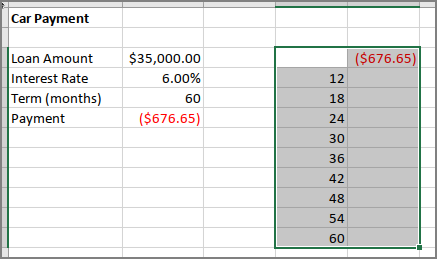
\includegraphics[width=\maxwidth{.95\linewidth}]{gfx/ch07_fig45}
	\caption{Preparing To Create a Data Table}
	\label{07:fig45}
\end{figure}

\begin{enumerate}[resume]	
	\item Click \fmtRibbonButton{Data Table} in the \fmtRibbonButton{What-If Analysis} button in the \fmtRibbonGroup{Forecast} group on the \fmtRibbonTab{Data} tab.
\end{enumerate}

\begin{figure}[H]
	\centering
	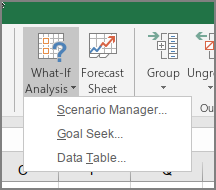
\includegraphics[width=\maxwidth{.95\linewidth}]{gfx/ch07_fig46}
	\caption{The What-If Analysis Menu}
	\label{07:fig46}
\end{figure}

\begin{enumerate}[resume]	
	\item In the \fmtPopupBox{Data Table} properties, enter \fmtTyping{\$B\$5} for Column input cell (leave the Row input cell blank since this data table has only one column with no rows). Excel will substitute values from \fmtCellLocation{D4:D12} into cell \fmtCellLocation{B5} one at a time and find the result using the formula in \fmtCellLocation{E3}.
\end{enumerate}

\begin{figure}[H]
	\centering
	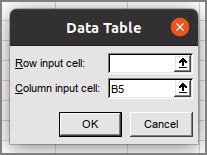
\includegraphics[width=\maxwidth{.95\linewidth}]{gfx/ch07_fig47}
	\caption{The Data Table Settings}
	\label{07:fig47}
\end{figure}

\begin{enumerate}[resume]	
	\item Click \fmtPopupButton{OK}.
\end{enumerate}

\begin{figure}[H]
	\centering
	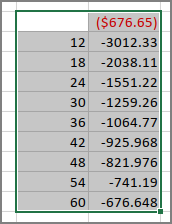
\includegraphics[width=\maxwidth{.95\linewidth}]{gfx/ch07_fig48}
	\caption{Data Table Results}
	\label{07:fig48}
\end{figure}

Riley should choose a term of $ 42 $ months since that creates the largest payment that is less than \$$ 1000 $. Note: the payments are negative numbers because they represent money that is leaving Riley's bank account.

In the one-variable example above only one variable, \textit{term}, was changed to determine its impact on the payment. Excel can also build a data table that reflects changing two variables. Imagine that Morgan is investing some savings in a fund that has an annual percentage rate of $ 5 $\%. Morgan can invest anywhere from \$$ 1000 $ to \$$ 10000 $ for any number of years from $ 2 $ to $ 7 $ and is interested to see how that investment will grow.

\begin{enumerate}
	\item Open \fmtWorkbookName{Advanced\_Exercises.xlsx}.
	\item Select the \fmtWorksheetName{Two Var Data Table} worksheet.
	\item Notice that some information has already been started, including the initial investment (cell \fmtCellLocation{B3}), annual percentage rate (cell \fmtCellLocation{B4}), number of compounding periods per year (\fmtCellLocation{B5}), and the number of years (cell \fmtCellLocation{B6}).
	\item Enter this formula to calculate the future value of the investment in cell \fmtCellLocation{B7}: \fmtTyping{=FV(B4/B5,B6*B5,,-B3)}. (Note, \textit{FV} Excel function that is used to calculate the future value of an investment. Note that there are two commas in a row and a negative sign before the last term.)
	\item In cell \fmtCellLocation{D3} enter: \fmtTyping{=B7}.
	\item In cell \fmtCellLocation{D4:D13} enter \fmtTyping{1000, 2000, 3000, 4000, 5000, 6000, 7000, 8000, 9000, 10000} (\textit{Tip}: using autofill may make this quicker).
	\item In cell \fmtCellLocation{E3:J3} enter \fmtTyping{2, 3, 4, 5, 6, 7}.
	\item Select \fmtCellLocation{D3:J13}.
\end{enumerate}

\begin{figure}[H]
	\centering
	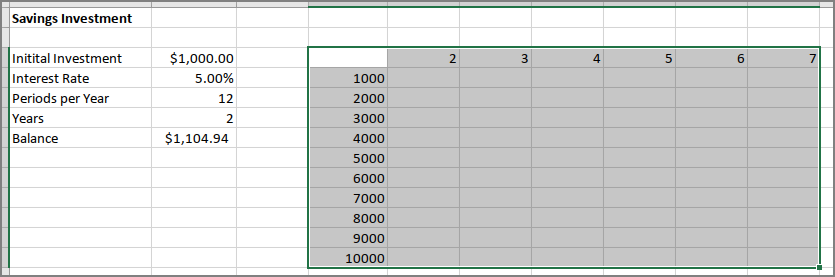
\includegraphics[width=\maxwidth{.95\linewidth}]{gfx/ch07_fig49}
	\caption{Two-Variable Data Table Setup}
	\label{07:fig49}
\end{figure}

\begin{enumerate}[resume]	
	\item Click \fmtRibbonButton{Data Table} in the \fmtRibbonButton{What-If Analysis} button in the \fmtRibbonGroup{Forecast} group on the \fmtRibbonTab{Data} tab.
	\item In the \fmtPopupBox{Data Table} properties, enter \fmtCellLocation{\$B\$6} for Row input cell and \fmtCellLocation{\$B\$3} for Column input cell.
	\item Click \fmtPopupButton{OK}.
\end{enumerate}

\begin{figure}[H]
\centering
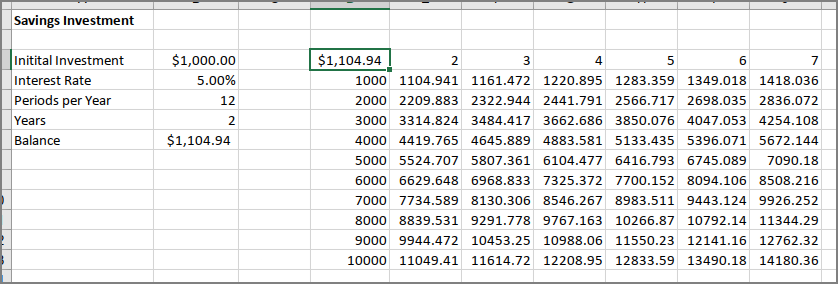
\includegraphics[width=\maxwidth{.95\linewidth}]{gfx/ch07_fig50}
\caption{Two-Variable Data Table Results}
\label{07:fig50}
\end{figure}

When Excel has completed the data table, Morgan would be able to balance the amount of money he can come up with initially with the length of time he is willing to leave that money in the bank.

\subsection{Goal Seek}

Often, business owners know the goal they seek for their company and they want Excel to determine how to achieve that goal. Imagine that a restaurant owner wants to know how much money to take in (``receipts'') to generate \$$ 100,000 $ in profit.

\begin{enumerate}
	\item Open \fmtWorkbookName{Ch7-Advanced.xlsx}.
	\item Select the \fmtWorksheetName{Goal Seek} worksheet.
	\item This worksheet already includes some data: the company receipts (\fmtCellLocation{B2}), the cost of food as a percentage of receipts (\fmtCellLocation{B3}), the overhead as a percentage of receipts (\fmtCellLocation{B4}), and a place for the net profit calculation (\fmtCellLocation{B5}).
	\item Enter this formula in \fmtCellLocation{B5}: \fmtTyping{=B2-((B2*B3)+(B2*B4))}.
	\item Click \fmtRibbonButton{Goal Seek} in the \fmtRibbonGroup{What-If Analysis} button in the \fmtRibbonGroup{Forcast} group on the \fmtRibbonTab{Data} tab.
	\item Enter \fmtTyping{\$B\$5} for the \textit{Set cell} parameter, enter \fmtTyping{$ 100,000 $} for the \textit{To value} parameter, and enter \fmtTyping{\$B\$2} for the \textit{By changing cell} parameter.
\end{enumerate}

\begin{figure}[H]
	\centering
	\includegraphics[width=\maxwidth{.95\linewidth}]{gfx/ch07_fig51}
	\caption{Goal Seek Setting}
	\label{07:fig51}
\end{figure}

\begin{enumerate}[resume]
	\item Click \fmtPopupButton{OK}.
\end{enumerate}

The data on the worksheet will adjust to fit the requirement. Clicking \fmtPopupButton{OK} on the \fmtPopupBox{Goal Seek Status} dialog box will change the worksheet while clicking \fmtPopupButton{Cancel} will revert the worksheet back to its original values.

\begin{figure}[H]
	\centering
	\includegraphics[width=\maxwidth{.95\linewidth}]{gfx/ch07_fig52}
	\caption{Goal Seek Results}
	\label{07:fig52}
\end{figure}

As a challenge, try using Goal Seek to change the overhead percentage in order to yield a profit of \$$ 35,000 $ with receipts of \$$ 100,000 $. 

\begin{center}
	\begin{tkwbox}{Key Take-Aways}
		\textbf{What-if Analysis}
		\\
		\begin{itemize}
			\setlength{\itemsep}{0pt}
			\setlength{\parskip}{0pt}
			\setlength{\parsep}{0pt}
			
			\item Data tables are effect ways to predict the effect of changes in a variable.
			\item Goal seeking finds an optimum value for a variable to meet a specific goal.
			
		\end{itemize}
	\end{tkwbox}
\end{center}

\section{Using Excel Macros}

\begin{center}
	\begin{objbox}{Learning Objectives}
		\begin{itemize}
			\setlength{\itemsep}{0pt}
			\setlength{\parskip}{0pt}
			\setlength{\parsep}{0pt}
			
			\item Automate simple tasks with a macro.
			
		\end{itemize}
	\end{objbox}
\end{center}

The \fmtRibbonButton{Macros} button in the \fmtRibbonGroup{Macros} group of the \fmtRibbonTab{View} tab allows users to automate repetitive tasks. The top part of the button will open the \fmtPopupBox{View Macros} dialog box and the bottom half reveals options for macros. 

\begin{enumerate}
	\item Open a new blank workbook. (\textit{Note}: the macro is placed in a new workbook so it does not accidentally interfere with the exercises in any other workbook.)
	\item Click \fmtCellLocation{A1} to select that cell.
	\item Click \fmtRibbonButton{Macros} in the \fmtRibbonGroup{Macros} group of the \fmtRibbonTab{View} tab (be sure to click the small arrow at the bottom of the \fmtRibbonButton{Macros} button).
	\item Select \fmtPopupButton{Use Relative References}.
	\item Select \fmtPopupButton{Record Macro}.
	\item Name the macro \fmtTyping{MyName}.
	\item Click in the \fmtPopupBox{Shortcut Key} box and type \fmtKeystroke{Shift} $ + $ \fmtKeystroke{Q}.
	\item Store the macro in this workbook.
	\item Enter this description: \fmtTyping{Inserts my name}.
\end{enumerate}

\begin{figure}[H]
	\centering
	\includegraphics[width=\maxwidth{.95\linewidth}]{gfx/ch07_fig53}
	\caption{The Record Macro Settings Box}
	\label{07:fig53}
\end{figure}

\begin{enumerate}[resume]	
	\item Click \fmtPopupButton{OK}.
	\item Type your first and last name and press \fmtKeystroke{Enter}.
	\item Click \fmtRibbonButton{Macros} in the \fmtRibbonGroup{Macros} group of the \fmtRibbonTab{View} tab (be sure to click the small arrow at the bottom of the \fmtRibbonButton{Macros} button).
	\item Select \fmtPopupButton{Stop Recording}.
\end{enumerate}

Select another cell on the worksheet and press \fmtKeystroke{Ctrl} $ + $ \fmtKeystroke{Shift} $ + $ \fmtKeystroke{Q}. Remember that relative references were activated for the macro, otherwise the name would have always been created in cell \fmtCellLocation{A1} (the original cell) instead of the current cell.

\begin{enumerate}
	\item Click \fmtRibbonButton{Macros} in the \fmtRibbonGroup{Macros} group of the \fmtRibbonTab{View} tab (be sure to click the top of the \fmtRibbonButton{Macros} button).
	\item This opens the Macro manager dialog where macros can be edited, deleted, or have various options set.
\end{enumerate}

\begin{figure}[H]
	\centering
	\includegraphics[width=\maxwidth{.95\linewidth}]{gfx/ch07_fig54}
	\caption{The Macro Manager Box}
	\label{07:fig54}
\end{figure}

\begin{enumerate}[resume]	
	\item Click \fmtPopupButton{Cancel} to close the Macro manager.
\end{enumerate}

Remember that all workbooks containing macros must be saved using the ``macro-enabled'' option (that creates a file extension of \textit{.xlsm}). Figure \ref{07:fig55} shows a drop-down menu at the bottom right corner of the \fmtPopupBox{Save-As} screen where \fmtPopupButton{Excel Macro-Enabled Workbook} must be selected. 

\begin{figure}[H]
	\centering
	\includegraphics[width=\maxwidth{.95\linewidth}]{gfx/ch07_fig55}
	\caption{Saving a Workbook With a Macro}
	\label{07:fig55}
\end{figure}

Since this macro will not be reused in the future, close the workbook without saving.

\begin{center}
	\begin{tkwbox}{Key Take-Aways}
		\textbf{Using Excel Macros}
		\\
		\begin{itemize}
			\setlength{\itemsep}{0pt}
			\setlength{\parskip}{0pt}
			\setlength{\parsep}{0pt}
			
			\item Macros automate simple tasks to save time in data entry.
			\item Workbooks containing macros must be saved with the ``Macro-Enabled'' setting.
			
		\end{itemize}
	\end{tkwbox}
\end{center}

\section{Preparing to Print}

\begin{center}
	\begin{objbox}{Learning Objectives}
		\begin{itemize}
			\setlength{\itemsep}{0pt}
			\setlength{\parskip}{0pt}
			\setlength{\parsep}{0pt}
			
			\item Review each worksheet in a workbook in Print Preview.
			\item Modify worksheets as needed to professionally print data and charts.
			
		\end{itemize}
	\end{objbox}
\end{center}

Just like consistency in formatting is important when working with workbooks containing multiple worksheets with pivot tables and charts,  so is consistency in page setup. Now that the \fmtWorkbookName{Sales Summary} workbook is complete, prepare it for printing by changing the adding a header and footer. 

\begin{enumerate}
	\item Open the \fmtWorkbookName{Sales Summary} workbook.
	\item Click \fmtPopupBox{Print} in the Backstage view to enter the print preview. To view all of the worksheets at one time, select \fmtPopupButton{Print Entire Workbook} in the first box in the Settings section. There are $ 6 $ pages to scroll through in Print Preview. At this point, clicking the \fmtPopupButton{Print} button would print all of the worksheets rather than just the active sheet.

	\begin{itemize}
		\item All of the pages look good except pages one and six.
		\item Page one is just the raw data. There is no point in printing that worksheet so it should be hidden.
		\item Page six should have a chart, but there is something wrong with that page.
		\item A header and footer should be added.
	\end{itemize}

	\item Exit Backstage View.
	\item Right-click on the \fmtWorksheetName{Sales Data} worksheet tab and select \fmtPopupButton{Hide}.
	\item Activate the \fmtWorksheetName{Sales By Item} worksheet by clicking that tab. Notice that part of the chart is printing on a second page as indicated by a dotted line running down the edge of column J. 
	\item Move and resize the chart so the top ``snaps'' to the top of Row $ 9 $, the bottom ``snaps'' to the bottom of Row $ 22 $, and the left side ``snaps'' to the left side of Column B. Resize right side of the chart so it snaps to the line between column F and G.
	\item Activate the \fmtWorksheetName{Sales Pivot} worksheet by clicking that tab. Hold down the \fmtKeystroke{Shift} key and click on the \fmtWorksheetName{Sales By Item} tab to activate all four worksheets.
	\item Click the \fmtRibbonButton{Page Setup} dialog box launcher arrow in the bottom right corner of the the \fmtRibbonGroup{Page Setup} group on the \fmtRibbonTab{Page Layout} tab then click the \fmtPopupButton{Header/Footer} tab.
	\item Click the \fmtPopupButton{Custom Footer} button. In the center section, insert the worksheet name using the \fmtPopupButton{Insert Sheet Name} button. The Footer dialog box should look like Figure \ref{07:fig56}.
\end{enumerate}

\begin{figure}[H]
	\centering
	\includegraphics[width=\maxwidth{.95\linewidth}]{gfx/ch07_fig56}
	\caption{Page Footer}
	\label{07:fig56}
\end{figure}

\begin{enumerate}[resume]	
	\item Click \fmtPopupButton{OK} to close the \fmtPopupBox{Footer} dialog box. 
	\item Click the \fmtPopupButton{Custom Header} button. In the right section, insert the date using the \fmtPopupButton{Insert Date} button. The Header dialog box should look like Figure \ref{07:fig57}.
\end{enumerate}

\begin{figure}[H]
	\centering
	\includegraphics[width=\maxwidth{.95\linewidth}]{gfx/ch07_fig57}
	\caption{Page Header}
	\label{07:fig57}
\end{figure}

\begin{enumerate}[resume]	
	\item Click \fmtPopupButton{OK} to close the \fmtPopupBox{Header} dialog box. 
	Click \fmtPopupButton{OK} again to close the \fmtPopupBox{Page Setup} dialog box.
	\item Return to Print Preview to confirm that each worksheet is printing on one page with the date appearing in the header and the correct worksheet name appearing in the footer.
\end{enumerate}

\begin{center}
	\begin{tkwbox}{Key Take-Aways}
		\textbf{Preparing to Print}
		\\
		\begin{itemize}
			\setlength{\itemsep}{0pt}
			\setlength{\parskip}{0pt}
			\setlength{\parsep}{0pt}
			
			\item Formatting for print is an essential part of creating a workbook.
			
		\end{itemize}
	\end{tkwbox}
\end{center}

\section{Chapter Practice}

\subsection{Project Team Analysis}

\textit{Data file: PR7-Data.csv}

\begin{enumerate}
	\item Load the data.

	\begin{enumerate}
		\item Start Excel and open a new workbook.
		\item Save the workbook as \fmtWorkbookName{Project}.
		\item Click \fmtRibbonButton{Get External Data} in the \fmtRibbonTab{Data} tab of the ribbon.
		\item Click \fmtPopupButton{From Text}. 
		\item Navigate to \fmtWorkbookName{PR7-Data.csv}.
		\item Click the file name and then \fmtPopupButton{Import}.
		\item Import the data file into a new worksheet.
	
		\begin{enumerate}
			\item The data in the CSV file has headers.
			\item The data uses a comma delimiter.
			\item The \textit{Date Completed} column should be formatted as \fmtPopupButton{Date MDY}.
			\item Import the data into cell \fmtCellLocation{A1} on the current worksheet.
		\end{enumerate}
	
		\item Name the worksheet \fmtWorksheetName{Project Data}.

	\end{enumerate}

	\item{\textbf{Question 1}: What type of project is the most fiscally productive?}

	\begin{enumerate}
		\item Activate cell \fmtCellLocation{A1} by clicking in the cell.
		\item Click \fmtRibbonButton{Recommended PivotTables} in the \fmtRibbonGroup{Tables} group of the \fmtRibbonTab{Insert} tab on the ribbon.
		\item Select the first pivot table, \fmtPopupButton{Sum of Amount Billed by Project Type} and click \fmtPopupButton{OK}.
		\item Rename the pivot table to \fmtTyping{Billed} and then rename the worksheet to \fmtTyping{Billed}.
		\item Move the \fmtWorksheetName{Billed} worksheet to the right of the \fmtWorksheetName{Project Data} worksheet.
		\item Click the down arrow to the right of \textit{Sum of Amount Billed} in the Values area and select \fmtPopupButton{Value Field Settings}.
		\item Change the name of this field to \fmtTyping{Total Billed}.
		\item Right-click in cell \fmtCellLocation{B4} to activate the first cell with totals.
		\item In the popup menu, select \fmtPopupButton{Sort} then \fmtPopupButton{Sort Largest to Smallest}. This sorts the total billed from the largest to smallest amount.
		\item Save the workbook.
	\end{enumerate}

	\item{\textbf{Question 2}: Which client spends the most?	}

	\begin{enumerate}
		\item Click in cell \fmtCellLocation{A1} in the \fmtWorksheetName{Project Data} worksheet to activate it.
		\item Click \fmtRibbonButton{PivotTable} in the \fmtRibbonGroup{Tables} group of the \fmtRibbonTab{Insert} tab.
		\item Create a pivot table on a new worksheet.
		\item Name the pivot table and worksheet \fmtTyping{Clients}.
		\item Move the \fmtWorksheetName{Clients} worksheet to the right of the \fmtWorksheetName{Billed} worksheet.
		\item Drag \textit{Client} from the Field List to the Rows area and \textit{Amount Billed} from the Field List to the Values area.
		\item Change the name of the values header from \textit{Sum of Amount Billed} to \fmtTyping{Total Billed}.
		\item Sort the \textit{Total Billed} column so the largest number is at the top.
		\item Save the workbook.
	\end{enumerate}

	\item{\textbf{Question 3}: Which quarter was the most profitable?}

	\begin{enumerate}
		\item Click in cell \fmtCellLocation{A1} in the \fmtWorksheetName{Project Data} worksheet to activate it.
		\item Click \fmtRibbonButton{PivotTable} in the \fmtRibbonGroup{Tables} group of the \fmtRibbonTab{Insert} tab.
		\item Create a pivot table on a new worksheet.
		\item Name the pivot table and worksheet \fmtTyping{Quarterly}.
		\item Move the \fmtWorksheetName{Quarterly} worksheet to the right of the \fmtWorksheetName{Clients} worksheet.
		\item Drag \textit{Data Completed} from the Field List to the Rows area and \textit{Amount Billed} from the Field List to the Values area.
		\item Change the name of the values header from \textit{Sum of Amount Billed} to \fmtTyping{Total Billed}.
		\item Save the workbook.
	\end{enumerate}
	
	\item{\textbf{Question 4}: Which team completed the largest proportion of the projects?}

	\begin{enumerate}
		\item Click in cell \fmtCellLocation{A1} in the \fmtWorksheetName{Project Data} worksheet to activate it.
		\item Click \fmtRibbonButton{PivotChart} in the \fmtRibbonGroup{Charts} group of the \fmtRibbonTab{Insert} tab.
		\item Create a pivot chart on a new worksheet.
		\item Name the pivot chart and worksheet \fmtTyping{Teams}.
		\item Move the \fmtWorksheetName{Teams} worksheet to the right of the \fmtWorksheetName{Quarterly} worksheet.
		\item Drag \textit{Team Leader} from the Field List to the \textit{Axis (Categories)} area and \textit{Hours Spent} from the Field List to the Values area.
		\item Change the name of the values header from \textit{Sum of Hours Spent} to \fmtTyping{Total Hours}.
		\item Sort the \textit{Total Hours} column so the largest number is at the top.
		\item Change the title of the chart to \fmtTyping{Total Hours Spent}.
		\item Since there is only one data point, the legend is not needed, so remove it. Click the $ + $ sign near the top right corner of the chart and uncheck the \fmtPopupButton{Legend} item.
		\item Save the workbook.
	\end{enumerate}

	\item Submit the \fmtWorkbookName{Project} workbook to the instructor.

\end{enumerate}

\section{Scored Assessment}

\subsection{Employee Analysis}

\textit{Data file: SC7-Data.csv}

\begin{enumerate}
	\item Load the data.
	
	\begin{enumerate}
		\item Start Excel and open a new workbook.
		\item Save the workbook as \fmtWorkbookName{Employees}.
		\item Click \fmtRibbonButton{Get External Data} in the \fmtRibbonTab{Data} tab of the ribbon.
		\item Click \fmtPopupButton{From Text}. 
		\item Navigate to \fmtWorkbookName{SC7-Data.csv}.
		\item Click the file name and then \fmtPopupButton{Import}.
		\item Import the data file into a new worksheet.
		
		\begin{enumerate}
			\item The data in the CSV file has headers.
			\item The data uses a comma delimiter.
			\item The \textit{hired} column (scroll to the right edge of the data list) should be formatted as \fmtPopupButton{Date MDY}.
			\item Import the data into cell \fmtCellLocation{A1} on the current worksheet.
		\end{enumerate}
		
		\item Name the worksheet \fmtWorksheetName{Employee Data}.
		
	\end{enumerate}
	
	\item{\textbf{Question 1}: What is the average salary for each role?}
	
	\begin{enumerate}
		\item Create a pivot table that lists the roles in the business (Accounting, Associate, etc.), the number of people in each role, and the average salary for that role.
		\item The pivot table should be on a worksheet named \fmtWorksheetName{Avr Salary} and that worksheet should be to the right of the \fmtWorksheetName{Employee Data} worksheet.
		\item The average salary should be formatted as currency. 
		\item Sort the list so the highest salary is first. 
		\item Save the workbook.
		\item Figure \ref{07:fig58} illustrates how the pivot table should look.
	\end{enumerate}

\end{enumerate}

\begin{figure}[H]
	\centering
	\includegraphics[width=\maxwidth{.95\linewidth}]{gfx/ch07_fig58}
	\caption{Avr Salary By Role}
	\label{07:fig58}
\end{figure}

\begin{enumerate}[resume]
	\item{\textbf{Question 2}: What is the average age of the employees when broken down by sex and marital status?}
	
	\begin{enumerate}
		\item Create a pivot table that lists the average age by marital status and sex for all employees.
		\item The pivot table should be on a worksheet named \fmtWorksheetName{Avr Age} and that worksheet should be to the right of the \fmtWorksheetName{Avr Salary} worksheet.
		\item The average age should be formatted as a number with two decimal places. 
		\item Save the workbook.
		\item Figure \ref{07:fig59} illustrates how the pivot table should look.
	\end{enumerate}
	
\end{enumerate}

\begin{figure}[H]
	\centering
	\includegraphics[width=\maxwidth{.95\linewidth}]{gfx/ch07_fig59}
	\caption{Avr Age}
	\label{07:fig59}
\end{figure}

\begin{enumerate}[resume]
	\item{\textbf{Question 3}: How many employees have been hired each year from 2007?}
	
	\begin{enumerate}
		\item Create a pivot table that lists the count by year. (\textit{Hint}: count the username field since each employee has a unique username.)
		\item The pivot table should be on a worksheet named \fmtWorksheetName{Year Hired} and that worksheet should be to the right of the \fmtWorksheetName{Avr Age} worksheet.
		\item The username field should be labeled \textit{count}. 
		\item The \textit{hired} field should display only years, not quarters or months.
		\item The list should be sorted by year (which is the default).
		\item Save the workbook.
		\item Figure \ref{07:fig60} illustrates how the pivot table should look.
	\end{enumerate}
	
\end{enumerate}

\begin{figure}[H]
	\centering
	\includegraphics[width=\maxwidth{.95\linewidth}]{gfx/ch07_fig60}
	\caption{Number Hired By Year}
	\label{07:fig60}
\end{figure}

\begin{enumerate}[resume]
	\item{\textbf{Question 4}: How many employees work in each role?}
	
	\begin{enumerate}
		\item Create a pivot chart that shows the count by role. (\textit{Hint}: count the username field since each employee has a unique username.)
		\item The pivot chart should be on a worksheet named \fmtWorksheetName{Count By Role} and that worksheet should be to the right of the \fmtWorksheetName{Year Hired} worksheet.
		\item The username field should be labeled \textit{Number}.
		\item The data should be sorted such that the role with the most employees (``Associate'') should be first.
		\item The chart's title should be \textit{Count By Role}
		\item The chart should not have a legend.
		\item Save the workbook.
		\item Figure \ref{07:fig61} illustrates how the pivot chart should look.
	\end{enumerate}
	
\end{enumerate}

\begin{figure}[H]
	\centering
	\includegraphics[width=\maxwidth{.95\linewidth}]{gfx/ch07_fig61}
	\caption{Count By Role}
	\label{07:fig61}
\end{figure}

\begin{enumerate}[resume]
	\item Submit the \fmtWorkbookName{Employees} workbook to the instructor.
\end{enumerate}